% ===== Speed toggle =====
\newif\ifdraft
\drafttrue            % <- set \draftfalse for final
\documentclass[\ifdraft draft\fi]{article}
\usepackage[margin=1.5in]{geometry}
\usepackage{amsmath, amsthm, amssymb}
\usepackage{xcolor}
\usepackage{enumitem}
\usepackage{sectsty}
\usepackage{float}
\usepackage{booktabs}
\usepackage{caption}
\usepackage{bm}
\usepackage[\ifdraft draft\else hidelinks\fi]{hyperref} % HYPERREF: disable link creation in draft (huge speedup)
\usepackage[\ifdraft draft\else final\fi]{graphicx} % Graphics: skip embedding in draft to speed up
\usepackage[most]{tcolorbox} % or consider 'framed' for lighter needs
\usepackage[round]{natbib}
\bibliographystyle{plainnat} % or an econ style you prefer (AER if you have it)
\usepackage{tikz}
\setlength{\parskip}{0.5em} % Add paragraph spacing
\sectionfont{\sectionrule{0pt}{0pt}{-4pt}{1pt}}
\subsectionfont{\sectionrule{0pt}{0pt}{-4pt}{.1pt}}
\newtheorem{proposition}{Proposition}
\tcbuselibrary{theorems} % Custom proof environment with light grey background
\newtcolorbox{greyproof} {colback=gray!10,colframe=gray!20,boxrule=0.5pt,arc=2pt,boxsep=3pt,left=6pt,right=6pt,top=6pt,bottom=6pt}

\title{A Knowledge-Sharing Model of Chatbots [SUPERCEDED]}
\author{Tom Cunningham}
\date{Sept 24 2025}

\begin{document}

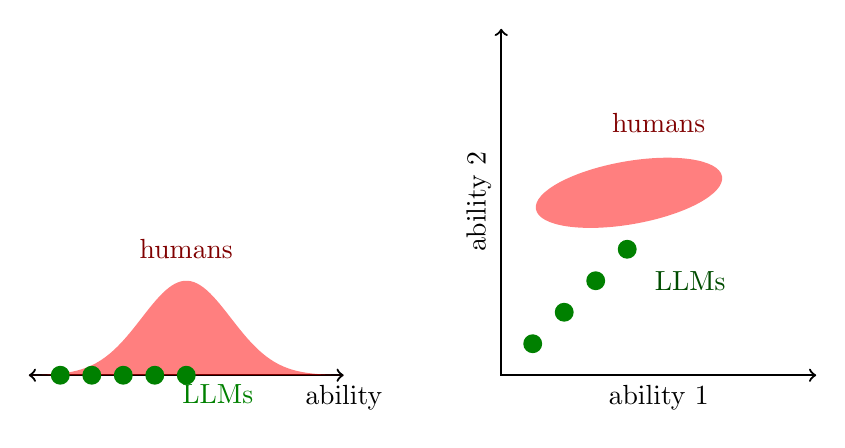
\begin{tikzpicture}[scale=4]
   % Left panel
   \begin{scope}      
      \draw[thick,<->] (1,0) node[right,below]{ability}  -- (0,0);
      \fill[red,opacity=0.5,thick,domain=0:1,samples=100] (0,0)-- plot(\x,{0.3*exp(-((\x-0.5)^2)/(0.2^2))}) -- (1,0) -- cycle;
      \node[red!50!black] at (.5,.4) {humans};

      \fill[green!50!black] (.1,0) circle(0.03);
      \fill[green!50!black] (.2,0) circle(0.03);
      \fill[green!50!black] (.3,0) circle(0.03);
      \fill[green!50!black] (.4,0) circle(0.03);
      \fill[green!50!black] (.5,0) circle(0.03);
      \node[green!50!black,below] at (.6,0) {LLMs};

   \end{scope}
   
   % Right panel
   \begin{scope}[xshift=1.5cm]
      \draw[thick,<->] (1,0) -- node[midway,below]{ability 1} (0,0)
         -- node[midway,rotate=90,above]{ability 2} (0,1.1);
      % \fill[green!50!black,opacity=0.5,rotate=65] (.3,-.2) ellipse (0.25 and 0.1);
      \fill[red,opacity=0.5,rotate=10] (.5,.5) ellipse (0.3 and 0.1);
      
      \node[red!50!black] at (.5,.8) {humans};
      % \draw[->,thick,green!50!black] (.26,.1)--(.45,.45);

      \fill[green!50!black] (.1,.1) circle(0.03);
      \fill[green!50!black] (.2,.2) circle(0.03);
      \fill[green!50!black] (.3,.3) circle(0.03);
      \fill[green!50!black] (.4,.4) circle(0.03);
      \node[green!30!black,align=left] at (.6,.3) {LLMs};
   \end{scope}
\end{tikzpicture}

\end{document}

